\documentclass[conference]{IEEEtran}
\IEEEoverridecommandlockouts
\usepackage[utf8]{inputenc}
\usepackage[T1]{fontenc}
\usepackage{amsmath,amssymb}
\usepackage{graphicx}
\usepackage{booktabs}
\usepackage{multirow}
\usepackage{xcolor}
\usepackage{algorithm}
\usepackage{algpseudocode}
\usepackage{tikz}
\usetikzlibrary{positioning,arrows.meta,fit,backgrounds}
\usepackage{url}
\usepackage{cite}

% Draft marker for the experiment section, which is pending additional runs.
\newcommand{\draft}[1]{\textcolor{red!70!black}{[DRAFT: #1]}}
\newcommand{\tbd}{\textcolor{red!70!black}{\textbf{TBD}}}

\begin{document}

\title{Hierarchical Evidence Pods: Structure-Preserving Hybrid Retrieval and Graph-Grounded Question Answering over Complex Technical Documents}

\author{\IEEEauthorblockN{Do Dang An}
\IEEEauthorblockA{Posts and Telecommunications\\Institute of Technology (PTIT)\\Hanoi, Vietnam}
\and
\IEEEauthorblockN{Dao Thi Thuy Quynh}
\IEEEauthorblockA{Posts and Telecommunications\\Institute of Technology (PTIT)\\Hanoi, Vietnam}}

\maketitle

\begin{abstract}
Question answering over technical manuals, specification sheets and contracts requires models to keep values attached to the right subject, table column, heading scope and footnote condition. Flat text chunking breaks these bindings, while feeding whole page images to vision--language models (VLMs) is costly and still leaves the binding implicit. We present a two-stage system that moves layout and structure analysis offline and hands the generator compact, explicitly scoped evidence. Offline, pages are rendered and analysed with Surya layout/OCR; tables are segmented with a Table Transformer and read cell by cell; GLiNER-RelEx proposes source-grounded entity spans; the result is projected into a per-document Neo4j graph (hierarchy, reading order, table rows/cells, figure--text candidates) and indexed with BM25, BGE-M3 and figure-level ColPali vectors. Online, a hybrid retriever fuses the three channels with reciprocal rank fusion, re-ranks them with a cross-encoder, selects seeds by question-part coverage and novelty, expands them inside the same document snapshot, and packages them as \emph{Hierarchical Evidence Pods}: sources grouped by document, reading stream and heading path, with table grids, merged-cell metadata, review warnings and stable citation IDs. Vision is used only offline and for retrieval (ColPali locates figures); the generator receives text only, so a language model without a vision encoder can answer from tables, footnotes and figures. On a 50-question pilot set over 20 technical documents, the production pipeline placed 95.6\% of gold evidence regions in the generator context. With text-only input to a zero-shot 7B generator, answer accuracy was 0.82, attribute leakage 4.8\% and citation faithfulness 0.92. In worked examples, structured OCR text was more accurate than full-page images (0.75 vs.\ 0.63) with about one fifth of the prompt tokens, and scope-aware graph expansion recovered missing evidence with 34--62\% fewer tokens than structural expansion.
\end{abstract}

\begin{IEEEkeywords}
document question answering, retrieval-augmented generation, table understanding, knowledge graph, hybrid retrieval, evidence packaging
\end{IEEEkeywords}

\section{Introduction}
Retrieval-augmented generation (RAG)~\cite{lewis2020rag} lets a language model answer from documents it was not trained on. Technical documents, however, are not running prose: product variants share one specification table, limits are qualified by footnotes, and the heading above a table decides which device a value belongs to. When such pages are cut into fixed-length text chunks, row--column alignment and heading scope disappear, and a generator can attach a value to the wrong subject---an error we call \emph{attribute leakage}. Reading the page image with a VLM~\cite{mathew2021docvqa,bai2025qwen25vl} keeps the layout but spends a large number of visual tokens per page and still leaves the model to infer which value belongs where.

This work takes a different position: the expensive structural analysis is done once, offline, and its result is preserved explicitly in the evidence given to the generator, \emph{as text}. The design goal is that a generator without a vision encoder can read tables, footnotes and figures correctly. Visual models are used where they are cheap and decisive---layout analysis and OCR offline, and ColPali as a \emph{retrieval} channel that locates relevant figures---while the online generator receives only structured text. The system (Fig.~\ref{fig:arch}) consists of an offline extraction stage (A3) and an online retrieval and answering stage (A2). Our contributions are:
\begin{itemize}
\item an offline pipeline that turns rendered pages into source-bound regions, cell-level table grids, figure--text candidates and a per-document graph, without letting similarity or model proposals become verified facts;
\item a hybrid retriever (BM25, BGE-M3, and figure-level ColPali used purely for retrieval; RRF; cross-encoder) with part-coverage and novelty-aware seed selection and snapshot-scoped graph expansion;
\item \emph{Hierarchical Evidence Pods}, an evidence serialization that groups sources by document, reading stream and heading path, renders verified table grids with merged-cell metadata, and keeps stable source IDs for checked citations;
\item an evaluation on a 50-question pilot set with frozen inputs, reporting the production pipeline with text-only generator input and worked examples for evidence format, graph expansion and visual input.
\end{itemize}

\section{Related Work}
\textbf{Document understanding.} LayoutLMv3~\cite{huang2022layoutlmv3} jointly models text and layout; DocVQA~\cite{mathew2021docvqa} benchmarks QA on page images. Surya~\cite{paruchuri2024surya} provides multilingual layout analysis, OCR and reading order, and the Table Transformer (TATR)~\cite{smock2022pubtables} detects table rows and columns. \textbf{Retrieval.} BM25~\cite{robertson2009bm25} remains strong for identifiers; BGE-M3~\cite{chen2024bgem3} provides multilingual dense embeddings; ColPali~\cite{faysse2025colpali} retrieves page images through late interaction over patch embeddings. Reciprocal rank fusion (RRF)~\cite{cormack2009rrf} combines rankings without score calibration. \textbf{Structure for LLMs.} GraphRAG~\cite{edge2024graphrag} builds entity graphs for corpus-level summarization; table serialization strongly affects LLM table understanding~\cite{sui2024table}; long contexts are used unevenly by LLMs~\cite{liu2024lost}. Our graph is per document and source-bound: it supplies scope and neighbours for retrieved regions rather than generated summaries. Query decomposition follows least-to-most prompting~\cite{zhou2023leasttomost}.

\section{Method}

\begin{figure*}[t]
\centering
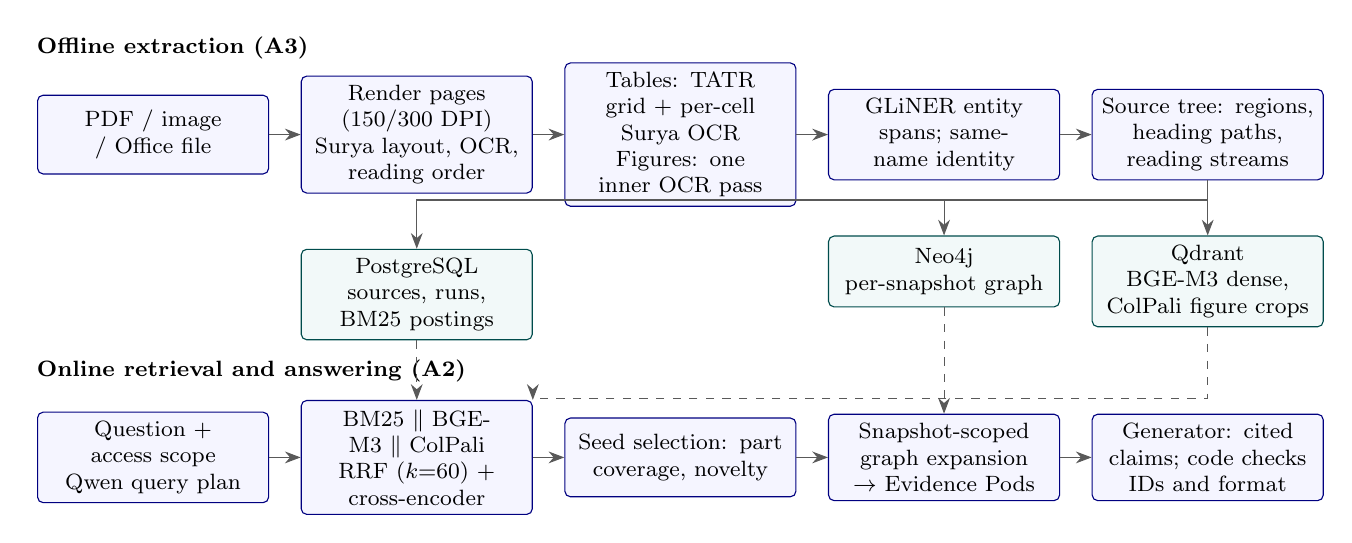
\begin{tikzpicture}[
  box/.style={draw=blue!50!black, fill=blue!4, rounded corners=2pt, align=center, font=\footnotesize, minimum height=10mm, text width=27mm},
  store/.style={draw=teal!60!black, fill=teal!5, rounded corners=2pt, align=center, font=\footnotesize, minimum height=9mm, text width=27mm},
  lab/.style={font=\footnotesize\bfseries, anchor=west},
  arr/.style={-{Stealth[length=2mm]}, gray!70!black}]
\node[lab] at (-1.6,1.1) {Offline extraction (A3)};
\node[box] (in) at (0,0) {PDF / image / Office file};
\node[box, right=4mm of in] (render) {Render pages (150/300 DPI)\\Surya layout, OCR, reading order};
\node[box, right=4mm of render] (table) {Tables: TATR grid + per-cell Surya OCR\\Figures: one inner OCR pass};
\node[box, right=4mm of table] (gliner) {GLiNER entity spans; same-name identity};
\node[box, right=4mm of gliner] (tree) {Source tree: regions, heading paths, reading streams};
\node[store, below=7mm of render] (sql) {PostgreSQL\\sources, runs, BM25 postings};
\node[store, below=7mm of gliner] (neo) {Neo4j\\per-snapshot graph};
\node[store, below=7mm of tree] (qd) {Qdrant\\BGE-M3 dense, ColPali figure crops};
\draw[arr] (in)--(render); \draw[arr] (render)--(table); \draw[arr] (table)--(gliner); \draw[arr] (gliner)--(tree);
\draw[arr] (tree.south) -- ++(0,-0.25) -| (sql.north); \draw[arr] (tree.south) -- ++(0,-0.25) -| (neo.north); \draw[arr] (tree)--(qd);
\node[lab] at (-1.6,-3.0) {Online retrieval and answering (A2)};
\node[box] (q) at (0,-4.1) {Question + access scope\\Qwen query plan};
\node[box, right=4mm of q] (ret) {BM25 $\|$ BGE-M3 $\|$ ColPali\\RRF ($k{=}60$) + cross-encoder};
\node[box, right=4mm of ret] (seed) {Seed selection: part coverage, novelty};
\node[box, right=4mm of seed] (pods) {Snapshot-scoped graph expansion $\rightarrow$ Evidence Pods};
\node[box, right=4mm of pods] (gen) {Generator: cited claims; code checks IDs and format};
\draw[arr] (q)--(ret); \draw[arr] (ret)--(seed); \draw[arr] (seed)--(pods); \draw[arr] (pods)--(gen);
\draw[arr, dashed] (sql.south) -- (ret.north); \draw[arr, dashed] (qd.south) -- ++(0,-0.9) -| (ret.north east); \draw[arr, dashed] (neo.south) -- (pods.north);
\end{tikzpicture}
\caption{System overview. Structural analysis is performed once offline; the online stage retrieves source regions and serializes them with their scope.}
\label{fig:arch}
\end{figure*}

\subsection{Offline extraction (A3)}
\textbf{Page rendering and layout.} Each PDF page is rendered twice, at 150\,DPI for page analysis and at 300\,DPI for text inside figures and for table structure; the PDF text layer is not used, so scanned and born-digital files follow the same path. Word, PowerPoint and spreadsheet files are parsed natively, keeping their own tables and embedded images. Surya~2~\cite{paruchuri2024surya}, a compact vision--language OCR model that we serve locally with llama.cpp, reads the page in a single full-page pass that returns layout regions (title, paragraph, list, table, figure, caption, header/footer, footnote), their text and their reading order. Each region becomes one \emph{source} carrying its text, page number and bounding box. A crop whose decoding loops or exhausts its token budget is retried once with wider framing and a larger budget; figure-text crops get one further low-temperature, contrast-enhanced attempt. Regions that still fail stay flagged and are excluded from retrieval and entity extraction, and a document with a failed page is not published to the graph.

\textbf{Tables.} Table regions are cropped from the 300\,DPI rendering. TATR~\cite{smock2022pubtables} (\texttt{table-transformer-structure-recognition}, a DETR detector with a ResNet-18 backbone) predicts columns, rows and spanning cells, which are reconciled with ruling lines visible in the crop, and every non-empty cell is read separately by Surya OCR (one enlarged retry for empty readings). The grid is accepted as \emph{cell-aware} only if it is complete and consistent---no holes, no overlapping cells, spans inside the grid, at most 200$\times$64 cells; the source text is then rebuilt from the cells, header rows and merged cells are stored as metadata, and the page OCR is kept for audit. Otherwise the table is \emph{unresolved}: no row/column text is published for it, and it can reach a generator only as an image crop.

\textbf{Figures.} Each page-level figure gets exactly one extra layout and OCR pass on its 300\,DPI crop. Page text overlapping the figure is masked first so that it keeps its own owner, and nested pictures are not scanned again. Every text region found inside becomes its own source, a child of the figure with a separate reading scope, marked as single-pass OCR. A caption that Surya places inside the figure region is attached to it; nearby captions and paragraphs are only linked by geometry as \emph{candidates} (\texttt{FIGURE\_CAPTION\_CANDIDATE}, \texttt{FIGURE\_NEAR\_TEXT\_CANDIDATE}), because proximity does not prove that a caption describes a figure. No free-form image description is generated.

\textbf{Hierarchy.} Heading levels are taken only from the model output or the native file; a heading with an unknown level is placed directly under the document rather than at a guessed depth. Tables, figures and their children are nested under the current heading, whereas page headers, footers and footnotes are attached to the document root. Sources are ordered by Surya's ranks within each page or figure scope; if the ranks are missing or ambiguous, the heading stack is reset instead of guessing an order.

\textbf{Entities.} GLiNER-RelEx (multilingual v1.0)~\cite{zaratiana2024gliner} is used for named-entity spans only (organisations, people, products and models, components, protocols), collapsed into a single entity type. A batch is accepted only if every span reproduces the source text exactly at its offsets, does not overlap another span and scores at least 0.5; relation output is rejected at this stage. Accepted spans become \texttt{MENTIONS} edges, and mentions with the same name inside one document are linked to one entity only when a GLiNER2 classifier judges them to denote the same thing in context. Model-proposed relations between passages are not published. The language model is not used in this stage.

\textbf{Related passages.} For every source, BGE-M3 proposes five similar sources in the same document; a pair becomes a \texttt{RELATED\_PASSAGE} edge only if the cross-encoder logit is non-negative and a GLiNER2 topic check agrees, with at most two links per source. These edges support navigation and are never treated as references.

\textbf{Graph projection.} Each extraction run is projected into Neo4j as a snapshot keyed by tenant, contract, version, run and source fingerprint; edges never cross snapshots. Node categories are \texttt{structure} (document and section headings), \texttt{layout\_block}, \texttt{evidence} (one per source region), \texttt{table}/\texttt{table\_row}/\texttt{table\_cell}, \texttt{source\_image}, \texttt{visual\_object}, \texttt{visual\_embedding} and \texttt{entity}. Edges include \texttt{CONTAINS} (heading hierarchy), \texttt{HAS\_EVIDENCE} (block to source), \texttt{NEXT} (reading order, created only between distinct unambiguous ranks within one page scope), \texttt{HAS\_ROW}/\texttt{HAS\_CELL}, \texttt{ABOVE}/\texttt{LEFT\_OF} (geometry only), figure--text candidates, \texttt{MENTIONS} and \texttt{RELATED\_PASSAGE} (embedding similarity candidates, never treated as verified references).

\textbf{Indexes.} Three retrieval indexes are built per version (ColPali serves retrieval only; its vectors are never given to the generator): a BM25~\cite{robertson2009bm25} index over token postings stored in PostgreSQL; 1024-dimensional BGE-M3~\cite{chen2024bgem3} dense vectors of source regions in Qdrant; and ColPali (\texttt{vidore/colpali-v1.2})~\cite{faysse2025colpali} multi-vectors computed only for figure crops. Text and table regions never fall back to full-page visual embeddings. Each figure vector is linked to its layout block in the graph through \texttt{HAS\_EMBEDDING}.

\textbf{Role of ColPali.} ColPali embeds the figure image itself: its vision encoder turns the crop into patch-level vectors, and a text query is scored against them by late interaction (MaxSim over query tokens and patches). It plays two roles. (1) \emph{Text-to-image search}: a question can reach a diagram, wiring drawing or labelled photo even when the figure's OCR text is sparse, misread or worded differently from the question. (2) \emph{Bridge from figures to text}: a retrieved figure is not passed to the generator as pixels; instead the graph connects it to the document's passages. Its in-figure text regions (\texttt{HAS\_FIGURE\_TEXT}) carry \texttt{MENTIONS} of entities, and passages elsewhere in the document that mention the same entities are added as context (\texttt{visual\_text\_shared\_entity\_candidate}), together with caption candidates. The generator thus receives the figure as its OCR text, caption candidates and the passages that discuss the same components, all as text.

\subsection{Online retrieval (A2)}
\textbf{Query planning.} In one call, the generator (Qwen2.5-VL-7B-Instruct, AWQ, served with vLLM~\cite{bai2025qwen25vl,kwon2023vllm}) splits the question into answer parts with retrieval queries, the reading scope and whether images are needed. If planning fails, retrieval uses the original question and records the planner as unavailable.

\textbf{Hybrid retrieval and fusion.} Every retrieval query is sent to all three channels over the latest versions the user may read. Candidate lists are fused with equal-weight RRF~\cite{cormack2009rrf},
\begin{equation}
\mathrm{RRF}(d)=\sum_{m\in\{\mathrm{BM25},\,\mathrm{dense},\,\mathrm{ColPali}\}}\frac{1}{60+r_m(d)},
\end{equation}
where $r_m(d)$ is the rank of $d$ in channel $m$ (terms are omitted when $d$ is absent). All fused candidates are then scored together by the multilingual cross-encoder \texttt{BAAI/bge-reranker-v2-m3}, always paired with the original request.

\textbf{Seed selection.} Seeds are chosen greedily. Let $P_i$ be the answer parts that candidate $i$ was retrieved for, $C$ the parts already covered, $\rho_i=\max_r 1/(1+\log_2 r)$ over its ranks, $o_i$ its maximum token Jaccard overlap with already selected seeds and $D$ the set of documents already used. The next seed maximizes, lexicographically,
\begin{equation}
\bigl(\,|P_i\setminus C|,\;\rho_i-0.35\,o_i+0.05\,[\mathrm{doc}_i\notin D],\;\textstyle\sum_r 1/(60+r)\bigr),
\end{equation}
up to $\min\!\bigl(24,\max(|\text{parts}|,\,3\cdot\text{groups})\bigr)$ seeds. Similar passages are down-weighted rather than discarded, so different versions, quantities and conditions remain available.

\textbf{Graph expansion.} For each seed, Neo4j returns neighbours within the same snapshot: sources reached through a direct structural relation of the seed's block (excluding the document root), sources sharing an entity mention, figure-text and visual-explanation links, and \texttt{RELATED\_PASSAGE} neighbours. Similarity-only neighbours are admitted only if they pass re-ranking against the question. Expanded sources are deduplicated and ordered by reading position.

\subsection{Hierarchical Evidence Pods}
Selected sources are serialized as pods (Algorithm~\ref{alg:pods}, Fig.~\ref{fig:pod}).
\begin{enumerate}
\item \textbf{Scope grouping.} Sources sharing document, version, file name, reading stream and heading path form one pod, printed once as a header (``Source scope $k$ \textbar{} Document/version $j$ \ldots{} Heading: A $>$ B $>$ C''). The heading path is fixed at extraction time from the source tree.
\item \textbf{Table grids.} Cell-aware tables are rendered as Markdown grids. Header rows are declared; if no header was detected, neutral column labels are used instead of guessing one. Merged cells are \emph{not} duplicated: they are listed as span metadata, so the model is told which cells span rows or columns rather than receiving copied values that the source does not repeat. An unresolved table carries no row/column text, only its status and the reason it was rejected.
\item \textbf{Figures.} Figure sources carry their in-image text, caption and location; figure--text links are presented as proposals.
\item \textbf{Links and IDs.} Each source keeps a stable ID (version, run, region). Graph links between selected sources are listed once next to their first source with direction and review status; structural machinery such as \texttt{HAS\_CELL} is not serialized.
\end{enumerate}
The generator returns claims (subject, attribute, value, condition, source IDs). Code checks that every cited ID was supplied and that the format is valid, with a single format-repair retry; it does not verify semantic correctness. If the prompt exceeds the context window (16{,}384 tokens), the output budget is reduced first and sources are then split into groups whose findings are combined against the original cited sources. The pods are plain text: a figure retrieved through ColPali reaches the generator as its in-image OCR text, caption candidates and location, so the answering step needs no vision encoder. The deployed system can optionally attach the figure or unresolved-table crop when the generator is a VLM; this option is disabled in all text-input experiments, and image input is studied only in E4.

\begin{algorithm}[t]
\caption{Evidence pod serialization}\label{alg:pods}
\begin{algorithmic}[1]
\Require selected sources $S$ (ordered), graph context $G$
\State $\mathcal{P}\gets$ ordered map from scope to list
\For{$s \in S$}
  \State $h\gets$ heading path of $s$; drop last element if $s$ starts with it
  \State $\kappa\gets(\text{doc},\text{version},\text{name},\text{reading stream},h)$
  \State $r\gets\{\text{id}(s)\}$; add review/OCR/table warnings
  \If{$s$ is a table and cells reproduce its OCR text}
    \State $r.\text{grid}\gets$ rows; $r.\text{header}\gets$ header rows; $r.\text{spans}\gets$ merged cells
  \Else \State $r.\text{text}\gets$ text of $s$ \EndIf
  \State append $r$ to $\mathcal{P}[\kappa]$
\EndFor
\State $L\gets$ edges of $G$ between selected sources (semantic, figure, similarity)
\State \Return render($\mathcal{P}$, $L$)
\end{algorithmic}
\end{algorithm}

\begin{figure}[t]
\centering
\footnotesize
\begin{tabular}{@{}p{0.95\columnwidth}@{}}
\toprule
\texttt{\#\# Source scope 1 | Document/version 1: LPH\_E}\\
\texttt{Heading: LPH\_E > Specifications}\\
\texttt{\#\#\# [a3:v1000015:r1000028:block:1001808]}\\
\texttt{\{"table\_header\_rows":[1],"merged\_cells":[\{"row":4,}\\
\texttt{\ \ "column":1,"rowspan":4,"colspan":1\}, \ldots]\}}\\
\texttt{| Term | | Specifications |}\\
\texttt{| --- | --- | --- |}\\
\texttt{| Motion angle | J1(1st-Axis) | ±130° |}\\
\texttt{| | J2(2nd-Axis) | ±146.6° |}\\
\texttt{| Maximum payload | | 3kg |}\\
\texttt{| Cycle time (*2) | | 0.45sec |}\\
\texttt{\#\#\# [a3:v1000015:r1000028:block:1001810]}\\
\texttt{*2 : Time required for a robot to move}\\
\texttt{a 2kg payload between two points 300 mm}\\
\texttt{apart at a height of 25mm.}\\
\bottomrule
\end{tabular}
\caption{Excerpt of an evidence pod produced by the system (abridged; ``Motion angle and stroke'' shortened). The merged motion-angle cell is declared as a span instead of being copied into each row. Here the cycle-time note was read as a paragraph under the same heading and therefore shares the table's scope.}
\label{fig:pod}
\end{figure}

\section{Experimental Protocol and Results}
\subsection{Setup}
\textbf{Corpus and questions.} The deployed index contains 201 document versions. The pilot set has 50 questions on 20 English technical documents (robot, controller, spark-plug, A/C service and wiper product literature) with reference answers, subject--attribute--value--condition tuples and gold evidence regions (65 regions, 16 tables). Categories: condition 31, table 18, comparison 13, footnote 11, procedure 7, identifier 5, figure text 3, multi-document 2. Gold answers were checked against the evidence text. The documents were also used during development, so the set is a pilot rather than an independent test set.

\textbf{Inputs are frozen.} Retrieval is run once with the production pipeline over all 201 versions (top-10 \texttt{query\_match} sources per question), and graphs are exported from Neo4j before any generation. Regions duplicated across uploads of the same PDF are matched by content hash in another version.

\textbf{Hardware.} The generator and ColPali are served on two NVIDIA Tesla T4 GPUs (15\,GB each; 10.0\,GB and 5.9\,GB in use while serving); vLLM runs with a memory utilisation of 0.8, giving a KV-cache pool of 38{,}448 tokens. Extraction models (Surya, TATR, GLiNER, BGE-M3 and the reranker) run on a local RTX~3050 Ti laptop GPU with 4\,GB.

\textbf{Generation.} Qwen2.5-VL-7B-Instruct-AWQ on vLLM ($16{,}384$-token context), temperature 0, max 2048 output tokens, one run per configuration (with temperature 0, 62 of 71 ablation configurations that were repeated gave identical outputs). The production main flow uses the deployed prompts and checks; the controlled ablations use a fixed JSON-schema output whose citation field is restricted to the supplied IDs. Prompt tokens are counted with the served model's tokenizer (revision \texttt{536a357}) and checked against API usage; sources are never truncated or padded.

\textbf{Experiments.} \emph{E1 (evidence format)}: the same evidence, order and model under A flat text, B JSON, C Markdown tables, D C+breadcrumb, E full pods; with gold evidence and with top-5 retrieved evidence. \emph{E2 (graph expansion)}: fixed top-3 retrieved seeds, one 6{,}000-token ceiling, modes A none, B previous/next blocks, C structural (B + parent heading, siblings, figure--text links), D scope-aware (C restricted to the seed's heading scope). \emph{E4 (visual input)}: full-page images, evidence crops, OCR text only, and OCR+caption structured pods, on questions with tables or figures; visual tokens are measured as API prompt tokens minus the tokenizer count of the same messages without images.

\textbf{Metrics.} Evidence recall and precision over the first ten sources (R@10, P@10) and required-evidence recall over all sources sent to the generator; citation precision (cited sources that are gold) and citation recall (gold regions cited); key-value recall, the share of gold numbers and codes from the subject--attribute--value tuples that appear in the answer (strict string match); prompt tokens, visual tokens and latency. Retrieval, citation, key-value and cost metrics are computed deterministically from the logs. Answer accuracy (correct 1, partial 0.5, wrong or no answer 0; strict accuracy counts only correct answers), attribute leakage rate (claims that bind a value or condition to the wrong subject, over all claims) and citation faithfulness (claims stated by the sources they cite, over all claims) were labelled by reading every answer against its reference answer, tuples and gold evidence, following a fixed rubric; the reader is one of the authors, so the labels are not an independent human evaluation.

\subsection{Results}
\textbf{Production main flow.} Each pilot question was run once through the deployed pipeline (planner, hybrid retrieval, re-ranking, graph expansion, evidence pods, checked generation) with text-only generator input (Table~\ref{tab:mainflow}). The generator is used zero-shot: no fine-tuning and no in-context examples, only the deployed instructions. Results are reported on the 45 questions with a completed answer.

\textbf{Retrieval.} The hybrid retriever ranked the gold regions within the first ten sources for 92\% of gold evidence (R@10; complete for 39 of 45 questions) and placed 95.6\% of them in the generator context after graph expansion (required-evidence recall). P@10 is 0.12 against a ceiling of 0.136, since a question has 1.36 gold regions on average: the context is deliberately broader than the minimal evidence. All 45 answers cite only source IDs that were supplied to the model. ColPali returned figure candidates for every question; 22\% of the top-ten sources (111 of 498, in 35 of 50 questions) were found by ColPali alone and by neither text channel, and the figure-to-text bridge added 52 passages in 10 questions. In this pilot no gold region arrived only through the visual channel: the three figure questions are answered by text inside the figures, which the text channels already find, so the pilot does not yet measure the benefit of visual search on diagrams without readable text.

\textbf{Citations.} 86\% of cited sources were gold regions (citation precision) and 84\% of gold regions were cited (citation recall).

\textbf{Answer quality.} The generator answered 31 of 45 questions correctly and 12 partially, with one wrong answer and one abstention (accuracy 0.82, strict 0.69); only 4.8\% of its claims bound a value to the wrong subject or condition, and 92\% of claims were stated by the sources they cited. Most partial answers omit one requested detail of a multi-part question rather than state something false.

\textbf{Text-only reading.} With text-only input, answers reproduced 84\% of gold numbers and codes (key-value recall over the 20 questions whose tuples contain such values; 15 of 20 complete), including all identifier questions and 87\% on table questions, without any image reaching the generator. This supports the design goal that the answering step does not need vision.

\textbf{Error analysis.}\label{sec:errors} We read the five text-only answers below full key-value recall. Two are correct and are missed by the strict string match (P044 gives ``+110, $-$102'' without the degree sign; P005 writes ``2,000 W''). Two are incomplete rather than wrong: P037 states the 25\,mm height of the cycle-time footnote but omits the 2\,kg load and 300\,mm distance, and P034 names the robots and arm count but not the RC8A controller. In P009 the footnote holding the answer was not retrieved, and the model stated that the documents do not cover the case instead of inventing a value. Footnote and condition questions are therefore the weakest group (62\% and 76\% key-value recall), consistent with the limitation that qualifiers are only linked to the values they modify when they are retrieved together. None of the five answers attached a value to the wrong subject.

% From research_evaluation_20261030/KET_QUA_20261030/{mainflow_manual_grades_summary,mainflow_retrieval_citation_summary,mainflow_summary}.csv (images off).
\begin{table}[t]
\centering\footnotesize
\caption{Production main flow on the 45 answered pilot questions (text-only generator input, zero-shot, one run). The P@10 ceiling is 0.136 because a question has 1.36 gold regions on average. Answer labels come from manual reading against reference answers, tuples and gold evidence.}
\label{tab:mainflow}
\setlength{\tabcolsep}{4pt}
\begin{tabular}{@{}lc@{\hspace{14pt}}lc@{}}
\toprule
\multicolumn{2}{@{}l}{\emph{Retrieval}} & \multicolumn{2}{l}{\emph{Answers}} \\
\midrule
Evidence recall@10 & 0.92 & Answer accuracy (partial = 0.5) & 0.82 \\
Evidence precision@10 & 0.12 & Strict accuracy & 0.69 \\
Required-evidence recall & 0.96 & Correct / partial / wrong / none & 31/12/1/1 \\
Sources sent per question & 31.6 & Attribute leakage rate $\downarrow$ & 0.048 \\
Citation precision & 0.86 & Citation faithfulness & 0.92 \\
Citation recall & 0.84 & Key-value recall (20 questions) & 0.84 \\
\bottomrule
\end{tabular}
\end{table}


\textbf{Worked examples.} The controlled ablations (fixed evidence and generator prompt) are reported on four questions each, namely those for which every configuration had completed; they illustrate behaviour and are not powered for significance. In E2 (Table~\ref{tab:e2}), expansion matters when retrieval misses part of the evidence: for P007 the seeds held one of two gold regions (R@10 0.50) and a single previous/next step recovered the other. Structural expansion admitted 13--28 sources and approached the 6{,}000-token ceiling, whereas scope-aware expansion rejected 17--96 candidates (mostly outside the seed's heading scope), kept the recovered evidence and used 34--62\% fewer tokens with 3.5--8.6$\times$ lower graph latency. In E4 (Table~\ref{tab:e4}), structured OCR text was at least as accurate as full-page images (0.75 vs.\ 0.63) with half the leakage, while using about one fifth of the prompt tokens (616 vs.\ 2{,}934; 2{,}760 visual tokens per page); region crops alone were the weakest input. All four inputs failed P040, whose table has a two-level header (standard specification vs.\ robot fitted with jacket): the models read the 7\,kg and 6\,kg values but bound them to the wrong configuration, which the key-value metric alone would have scored as correct. In E1 (Table~\ref{tab:e1}) the four examples are text questions without tables; all formats cited only gold sources and breadcrumbs gave the most complete citations with gold evidence, while full pods cost the most tokens without a gain on these questions. A full-scale E1 on table-heavy questions remains to be run.

% Worked examples from research_evaluation_20261030/KET_QUA_20261030/{E1,E2,E4}_examples.csv (one run per cell).
% Examples are the pilot questions for which every configuration had completed; not selected by outcome.
\begin{table}[t]
\centering\footnotesize
\caption{E2 graph expansion on four worked examples (top-3 retrieved seeds, 6{,}000-token ceiling). +N: sources added; Rej.: candidates rejected (scope boundary, token budget, empty, duplicate); R/P@10: evidence recall/precision at 10; Graph ms includes tokenizer calls for the budget.}
\label{tab:e2}
\setlength{\tabcolsep}{2.5pt}
\begin{tabular}{@{}llcccccc@{}}
\toprule
Q & Mode & +N & Rej. & R@10 & P@10 & Tokens & Graph ms \\
\midrule
\multirow{4}{*}{P003} & A none & 0 & 0 & 1.00 & 0.33 & 1054 & 6 \\
 & B prev/next & 5 & 1 & 1.00 & 0.14 & 1934 & 38 \\
 & C structural & 22 & 1 & 1.00 & 0.10 & 5483 & 207 \\
 & D scope-aware & 6 & 17 & 1.00 & 0.12 & 2079 & 24 \\
\midrule
\multirow{4}{*}{P007} & A none & 0 & 0 & \textbf{0.50} & 0.33 & 810 & 5 \\
 & B prev/next & 3 & 3 & \textbf{1.00} & 0.33 & 1339 & 16 \\
 & C structural & 28 & 16 & 1.00 & 0.20 & 5895 & 345 \\
 & D scope-aware & 15 & 29 & 1.00 & 0.20 & 3468 & 98 \\
\midrule
\multirow{4}{*}{P022} & A none & 0 & 0 & 1.00 & 0.33 & 2181 & 7 \\
 & B prev/next & 4 & 0 & 1.00 & 0.14 & 3033 & 32 \\
 & C structural & 13 & 14 & 1.00 & 0.10 & 5965 & 308 \\
 & D scope-aware & 6 & 21 & 1.00 & 0.11 & 3739 & 52 \\
\midrule
\multirow{4}{*}{P027} & A none & 0 & 0 & 1.00 & 0.33 & 880 & 5 \\
 & B prev/next & 6 & 0 & 1.00 & 0.11 & 2158 & 36 \\
 & C structural & 24 & 86 & 1.00 & 0.10 & 5858 & 462 \\
 & D scope-aware & 14 & 96 & 1.00 & 0.10 & 3840 & 90 \\
\bottomrule
\end{tabular}
\end{table}

\begin{table}[t]
\centering\footnotesize
\caption{E4 visual input on four table/figure questions (P013, P028, P039, P040; gold evidence). Acc.: manual answer accuracy (partial 0.5); ALR: attribute leakage rate over claims; Cit.\ R: gold regions cited; tokens are means over questions. KV mem.: GPU KV-cache memory held by the prompt, computed as prompt tokens $\times$ 56\,KiB (Qwen2.5-VL-7B: 28 layers, 4 KV heads, head size 128, FP16); vision-encoder activations are not included. Offline extraction cost is shared by all inputs (median 19\,s per page for the whole A3 pipeline).}
\label{tab:e4}
\setlength{\tabcolsep}{2.5pt}
\begin{tabular}{@{}lcccccc@{}}
\toprule
Generator input & Acc. & ALR$\downarrow$ & Cit.\ R & Vis.\ tok. & Prompt tok. & KV mem. \\
\midrule
Full-page image (VLM) & 0.63 & 0.22 & 1.00 & 2760 & 2934 & 160\,MiB \\
Region crops (VLM) & 0.25 & 0.11 & 0.50 & 241 & 411 & 22\,MiB \\
OCR text only & \textbf{0.75} & \textbf{0.10} & 1.00 & 0 & 510 & 28\,MiB \\
OCR + caption pods (ours) & \textbf{0.75} & \textbf{0.10} & 1.00 & 0 & 616 & 34\,MiB \\
\bottomrule
\end{tabular}
\end{table}

\begin{table}[t]
\centering\footnotesize
\caption{E1 evidence format on four worked examples (P002, P018, P023, P029; mean over questions, one run). All cited sources were gold in every cell (citation precision 1.00). These four are text questions without tables, so formats differ mainly in length.}
\label{tab:e1}
\setlength{\tabcolsep}{3pt}
\begin{tabular}{@{}lcccc@{}}
\toprule
 & \multicolumn{2}{c}{Gold evidence} & \multicolumn{2}{c}{Retrieved (top-5)} \\
Format & Cit.\ R & Tokens & Cit.\ R & Tokens \\
\midrule
A flat text & 0.88 & 222 & 0.88 & 468 \\
B JSON & 0.75 & 240 & 0.88 & 531 \\
C Markdown table & 0.88 & 222 & 0.88 & 475 \\
D + breadcrumb & \textbf{1.00} & 265 & 0.88 & 617 \\
E full pods & 0.88 & 414 & 0.88 & 1088 \\
\bottomrule
\end{tabular}
\end{table}


\section{Discussion and Limitations}
\textbf{Structure as text.} The results support moving structure analysis offline. Once tables are delivered as grids and figure text as OCR with caption candidates, a 7B generator answered more accurately from text than from full-page images in our worked examples, at a fraction of the prompt length, and in the main flow it reached 0.82 accuracy with text alone. 

\textbf{Image input.} The generator is a 7B quantized VLM used zero-shot, so its reading of images reflects an untuned model rather than the value of visual evidence: given images alone it scored 0.63 on full pages and 0.25 on region crops, below the 0.75 it reached on structured text of the same evidence (Table~\ref{tab:e4}); crops in particular remove the labels and headings that the pods keep. We therefore treat images as an offline and retrieval resource in this work. Combining image crops with the pods for a VLM generator---for example, attaching a crop only where the pods lack text, such as unresolved tables---requires a stronger or adapted VLM and is left for future work.

\textbf{Scope over volume.} Graph expansion is most useful when retrieval returns part of the evidence. Adding every structural neighbour fills the budget with siblings that rarely matter; restricting expansion to the seed's heading scope kept the recovered evidence with far fewer tokens.

\textbf{Limitations.} (i) a table whose grid fails validation is published without text, so a text-only generator cannot read it and only an image crop remains, and even a valid grid with a two-level header (P040) can be misread because the header hierarchy is declared only as merged-cell metadata; (ii) regions labelled as footnotes are attached to the document root, so a footnote can land in a different pod from the table it qualifies and is used only when retrieval returns it as well; (iii) heading scope can be wrong when contact blocks at the page bottom are attached to the preceding heading; (iv) \texttt{RELATED\_PASSAGE} similarity links include noise (shared URLs, boilerplate) and are therefore presented only as proposals; (v) answers are checked for citation IDs and format, not by an independent semantic verifier; (vi) the pilot uses one generator, one run per configuration and documents seen during development, and the ablations are worked examples rather than full-scale comparisons; text-only conditions used Qwen2.5-VL without images rather than a model lacking a vision encoder. Future work extends the evaluation to 200--300 questions on unseen documents, a text-only LLM and full-scale format and expansion ablations.

\section{Conclusion}
We described a system that performs layout, table and figure analysis offline and gives the generator source regions together with their document, heading and reading-stream scope, explicit table grids and stable citation IDs. On a pilot set of technical documents the pipeline retrieved nearly all gold evidence, and a zero-shot generator given only structured text answered with accuracy 0.82, attribute leakage of 4.8\% and citation faithfulness of 0.92, while structured text outperformed full-page images at about one fifth of the prompt length. Vision is thus needed for building the evidence, not for reading it.

\textbf{Code and data availability.} The extraction and retrieval code, the evaluation scripts, the pilot questions with gold evidence and the per-question logs are available at \url{https://github.com/Andydo21/MultiModelAndExtract}.

\bibliographystyle{IEEEtran}
\bibliography{refs}

\end{document}
